%%%%%% CMB-S4 Inflation Chapter  %%%%%%%%%%%%%%%%
 
\chapter{Inflation Physics from the Cosmic Microwave Background}
%\renewcommand*\thesection{\arabic{section}}

%%%%%%%%%%%%%%%%%%%%%%%%%%%%%%%%%%%%%%%%%%%%%%%%%%%%%%%%%%%
%%%%%%%%%%%%%%%%%%%%%%%%%%%%%%%%%%%%%%%%%%%%%%%%%%%%%%%%%%%
%%%%%%%%%%%%%%%%%%%%%%%%%%%%%%%%%%%%%%%%%%%%%%%%%%%%%%%%%%%
%%%%%%%%%%%%%%%%%%%%%%%%%%%%%%%%%%%%%%%%%%%%%%%%%%%%%%%%%%%


\begin{center}
{\small {\it (send feedback on this chapter to \href{mailto:s4\_inflation@cosmo.uchicago.edu}{s4\_inflation@cosmo.uchicago.edu})}}
\end{center}



\section{Introduction}
%The study of the polarization of the cosmic microwave background will bring additional information about both the gravitational and matter sectors of the primordial universe. However, for primordial gravitational waves there are clear theoretical thresholds that can be reached with this next generation instrument. We will use the tensor-to-scalar ratio as the primary inflationary science driver for the design.

The small anisotropies in the cosmic microwave background radiation contain invaluable information about the primordial universe. On the one hand, they encode the properties of the primordial scalar (or density) perturbations and hence the matter sector of the primordial universe. 
%Models of the primordial universe make quantitative predictions for the statistical properties of primordial scalar perturbations, for example for their scale dependence. 
CMB-S4 will significantly improve current constraints on primordial observables in the scalar sector, typically by a factor of at least five. On the other hand, on degree scales a polarization pattern known as B-mode polarization would reveal the existence of primordial tensor modes or gravitational waves. In the tensor sector, CMB-S4 will improve current constraints by almost two orders of magnitude. This is especially interesting because it allows this next generation instrument to reach theoretically well-motivated thresholds for the tensor-to-scalar ratio (the ratio of power in tensor modes to power in scalar modes), which consequently serves as the primary inflationary science driver for the design. A detection of primordial gravitational waves in the range accessible to this instrument would:
\begin{itemize}
 \item Reveal a new scale of particle physics far above those accessible with terrestrial particle colliders.  
\item  Rule out the only currently developed competitor to inflation (ekpyrotic scenario)
\end{itemize}
If, in addition, we can conclusively determine that any detected signal is dominated by vacuum fluctuations then a detection would also
\begin{itemize}
 \item Identify the energy scale of inflation. 
 \item Provide strong evidence that the complete theory of quantum gravity must accommodate a Planckian field range for the inflaton.
 \item Provide strong evidence that gravity is quantized, at least at the linear level.
\item  Constrain the mass of the graviton
\end{itemize}
In the absence of a detection CMB-S4 will rule out large classes of inflation models. 

In Section \ref{sec:detection} we review in detail what a detection of primordial gravitational waves would mean and what follow-up measurements should or could be done to further characterize any signal. Section \ref{sec:upperLimits} explains the implications of a robust upper limit of $r<0.001$. Section \ref{sec:needs} lays out what is required to achieve that goal. The final two sections describe the significant gains CMB-S4 will allow in constraining other aspects of the primordial universe, both standard and more speculative. These include characterizing the scalar power spectrum, constraining curvature, non-Gaussianity, isocurvature modes, further probes of CMB `anomalies' and test/constraints of cosmic strings.
 
%Recent reviews \cite{Kamionkowski:2015yta}.

\section{Implications of a detection of primordial gravitational waves with CMB-S4}
\label{sec:detection}
The overall evolution of the universe is well modeled by a Friedmann-Lema\^{\i}tre-Robertson-Walker line element
\begin{equation}
ds^2=-dt^2+a^2(t)\left[\frac{dr^2}{1-kr^2}+r^2d\Omega^2\right]\,,
\end{equation}
where $k=\pm1$ allows for spatial curvature and the time evolution is specified by the scale factor, $a(t)$. The Hubble parameter, $H=\dot{a}/a$, gives the rate of expansion of the universe. 
%Current data is consistent with a spatially flat universe, and we will assume spatial flatness ($k=0$) for most of the discussion. However, we will return to constraints on the curvature in Section xxx.  

The existence of primordial Helium and the cosmic microwave background radiation provide strong evidence for a hot big bang, a period during which the universe was dominated by radiation before it became dominated by matter and eventually dark energy. In the context of general relativity, observations of the cosmic microwave background furthermore provide strong evidence for a period preceding the hot big bang during which the co-moving Hubble radius, $(a|H|)^{-1}$, was decreasing with time: the measured average CMB temperature and the statistics of the measured anisotropies are the same over regions that otherwise share no causal history. 

%Arguably the most significant discrepancy between the predictions of a generic hot big bang model and our observed sky is the horizon problem: the measured average CMB temperature and the statistics of the measured anisotropies are the same over regions that share no causal history. Models for the primordial universe attempt to give a causal (and ideally also a `natural') explanation for the observed homogeneity on scales greater than a few degrees by postulating an early era where the co-moving Hubble radius, $(a|H|)^{-1}$ is decreasing with time. In an expanding universe this requires an era of accelerated expansion, $\ddot{a}>0$. The matter field that sources this expansion should have equation of state $w\approx -1$, which is minimally provided by a single scalar field whose energy density is predominately determined by its potential.

In an expanding universe a decreasing co-moving Hubble radius requires an era of accelerated expansion, $\ddot{a}>0$, cosmic inflation. Such a period will drive the spatial curvature close to zero, in good agreement with current observations. Thus, we will assume spatial flatness and set $k=0$ for most of the discussion, but will return to constraints on the curvature in Section \ref{sec:other_topics}. Since the period of cosmic inflation must end, there must exist a clock, or scalar degree of freedom. According to the uncertainty principle this clock must fluctuate, generating density perturbations that are adiabatic. In the most economic scenarios, these density perturbations are the seeds that grow into the anisotropies observed in the cosmic microwave background radiation and the stars and galaxies around us. Other degrees of freedom could, of course, also be present during this phase and might even be responsible for the generation of density perturbations we observe. {\bf (Mention isocurvature modes here?)}

Alternatively, the phase of decreasing co-moving Hubble radius could have occurred during a period of decelerating contraction which must then be followed by a bounce as in the ekpyrotic or matter bounce scenarios. 
% The matter field that sources this expansion should have an equation of state $w\approx -1$, which is minimally provided by a single scalar field whose energy density is predominately determined by its potential.

%The remarkable feature of inflation is that once an evolving scalar field is invoked to source the background accelerated expansion, quantum fluctuations during inflation inevitably generate post-inflationary metric perturbations. 
For these early times, the ADM formalism provides a convenient parametrization of the line element
\begin{eqnarray}
\label{eq:metric}
ds^2&=&-N^2dt^2 +h_{ij}(dx^i+N^idt)(dx^j+N^jdt)\,\nonumber\\
h_{ij}&=&a^2(t)[e^{2\zeta}\delta_{ij}+\gamma_{ij}]\,.
\end{eqnarray}

The equations of motion for $N$ (the lapse) and $N^i$ (the shift) are the Hamiltonian and momentum constraints, while $\zeta$ ($=-\mathcal{R}$ of {\it Planck}) and $\gamma_{ij}$ contain the dynamical scalar and tensor degrees of freedom. In scenarios with matter sources other than a scalar field there may also be vector perturbations. These rapidly decay and can be neglected unless they are actively sourced in the post-inflationary universe, e.g. by cosmic strings.

%RF perhaps add Fourier transform and define horizon exit, freeze out at this point
Because the equations of motion are invariant under translations and the perturbations are linear or nearly so, it is convenient to work with the Fourier transforms
\begin{equation}
\zeta(t,\vec{x})=\int \frac{d^3 k}{(2\pi^3)}\zeta(t,\vec{k})e^{i \vec{k}\cdot\vec{x}}+h.c.\qquad{\rm and}\qquad\gamma_{ij}(t,\vec{x})=\sum\limits_s\int\frac{d^3k}{(2\pi^3)}\gamma_s(t,\vec{k})e_{ij}(\vec{k},s)e^{i \vec{k}\cdot\vec{x}}+h.c.\,,
\end{equation}
where $e_{ij}(\vec{k},s)$ is the transverse traceless polarization tensor for the graviton. The solutions oscillate when the modes are deep inside the horizon, $k\gg aH$. By definition, the modes exit the horizon when $k=aH$ and in single-field models approach a constant outside the horizon when $k\ll aH$.

The statistical properties of the scalar and tensor fluctuations, $\zeta$ and $\gamma_s$, at times sufficiently late so that they have frozen out provide the link between the primordial era and the CMB as well as other probes of the structure of the late universe. For a universe that is statistically homogeneous and isotropic and in which the primordial fluctuations are Gaussian, the information about the statistical properties is contained in the two-point correlation functions

\begin{eqnarray}
\langle\zeta(\vec{k})\zeta(\vec{k}^{\prime})\rangle&=&(2\pi)^3\delta^3(\vec{k}+\vec{k}^{\prime})\frac{2\pi^2}{k^3}\mathcal{P}_{\zeta}(k)\nonumber\\
\langle\gamma_s(\vec{k})\gamma_{s^{\prime}}(\vec{k}^{\prime})\rangle&=&(2\pi)^3\delta_{ss^{\prime}}\delta^3(\vec{k}+\vec{k}^{\prime})\frac{2\pi^2}{k^3}\frac{1}{2}\mathcal{P}_{t}(k)\nonumber\\
\end{eqnarray}
where the factor of $1/2$ in the second to last line accounts for the fact that the measured power includes contributions from each of the two graviton polarizations. In single field slow-roll inflation, the gauge invariant combination of metric and scalar field fluctuations that is conserved outside the horizon has the power spectrum
\begin{equation}
\label{eq:inf_Pzeta}
\mathcal{P}_{\zeta}(k)=\frac{1}{2\epsilon M_p^2}\left.\left(\frac{H}{2\pi}\right)^2\right|_{k=aH}
\end{equation}
where $\epsilon=-\dot{H}/H^2$ is the first slow-roll parameter, and $M_p=1/\sqrt{8\pi G}$ is the reduced Planck mass. As indicated, the Hubble parameter and $\epsilon$ are to be evaluated at horizon exit when the wavenumber $k$ is equal to the inverse comoving Hubble radius. In the absence of additional sources, the tensor power spectrum generated by inflation is
\begin{equation}
\label{eq:inf_Pt}
\mathcal{P}_{t}(k)=\frac{8}{M_p^2}\left.\left(\frac{H}{2\pi}\right)^2\right|_{k=aH}
\end{equation}

It is convenient to introduce the logarithmic derivatives of these power spectra 
\begin{equation}\label{eq:specind}
n_s(k)-1\equiv\frac{d\ln \mathcal{P}_{\zeta}}{d\ln k}\qquad{\rm and}\qquad n_t(k)\equiv \frac{d\ln \mathcal{P}_t}{d\ln k}\,.
\end{equation}
If the Hubble rate and slow-roll parameter only weakly depend on time as in slow-roll inflation, these will be $n_s(k)\approx 1$ and $n_t(k)\approx 0$ and can be expanded around a pivot scale $k_\star$ accessible by the CMB
\begin{equation}
n_s(k)-1=n_s-1+\left.\frac{dn_s(k)}{d\ln k}\right|_{k_\star}\ln(k/k_\star)+\dots\qquad{\rm and}\qquad n_t(k)=n_t+\left.\frac{dn_t(k)}{d\ln k}\right|_{k_\star}\ln(k/k_\star)+\dots
\end{equation}
In this approximation, the power spectra are
\begin{eqnarray}
\mathcal{P}_{\zeta}(k)&=& A_s\left(\frac{k}{k_\star}\right)^{n_s-1+\frac{1}{2}\left.\frac{dn_s}{d\ln k}\right|_{k=k_\star}\ln(k/k_\star)+\dots}\,,\nonumber\\
\mathcal{P}_{t}(k)&=& A_t \left(\frac{k}{k_\star}\right)^{n_t+\frac{1}{2}\left.\frac{dn_t}{d\ln k}\right|_{k=k_\star}\ln(k/k_\star)+\dots}\,,
\end{eqnarray}
%\begin{equation}\label{eq:specind}
%\mathcal{P}_{\zeta}(k)\equiv A_s\left(\frac{k}{k_\star}\right)^{n_s-1}\qquad{\rm and}\qquad\mathcal{P}_{t}(k)\equiv A_t \left(\frac{k}{k_\star}\right)^{n_t}\,,
%\end{equation}
where $A_s$, $A_t$ are the scalar and tensor amplitudes, and $n_s$ and $n_t$, are the scalar and tensor spectral index, respectively, both at the pivot scale. 
The tensor-to-scalar ratio, $r$, is the relative power in the two types of fluctuations at a chosen pivot scale $k_\star$ accessible by the CMB
\begin{equation}
r=\frac{A_t}{A_s}
\end{equation}

The power spectra of $\zeta$ and $\gamma_s$ are time-independent as long as the modes are outside the horizon, and only begin to evolve once the modes of interest re-enter the horizon at late times. In particular, they set the initial conditions for the system of equations governing the time evolution of the universe from around $10^9$ K when electrons and positrons have annihilated to the present. To exhibit the link between the primordial perturbations and late time observables explicitly, note that in a spatially flat universe, the contributions of primordial scalar perturbations to the angular power spectra of temperature or E-mode anisotropies are given by
\begin{equation}
C^{(S)}_{XX,\ell}=\int \frac{dk}{k}\mathcal{P}_\zeta(k)\left|\int\limits_0^{\tau_0} d\tau S_X^{(S)}(k,\tau)j_\ell(k(\tau_0-\tau))\right|^2\,,
\end{equation}
where $S_X^{(S)}(k,\tau)$ with $X=T,E$ are source functions that encode the physics of recombination and $j_\ell$ is a spherical Bessel function that encodes the (spatially flat) geometry of the universe.
% and $\mathcal{P}_\zeta(k)$ is the power spectrum of initial conditions of primordial scalar perturbations as a function of the (comoving) momentum of the modes. 
At linear order, scalar perturbations only contribute to angular power spectra of temperature and E-mode polarization and the cross-spectrum of temperature and E-mode polarization, while the tensor perturbations in addition generate B-mode polarization. The primordial contribution of the tensor perturbations to the angular power spectrum of B-modes is 
\begin{equation}
C_{BB,\ell}=\int \frac{dk}{k}\mathcal{P}_t(k)\left|\int\limits_0^{\tau_0} d\tau S_B^{(T)}(k,\tau)j_\ell(k(\tau_0-\tau))\right|^2\,.
\end{equation}
where $S_B^{(T)}(k,\tau)$ is the appropriate source function. 

At present, bounds on the tensor contribution to the temperature and E-mode anisotropies are comparable to constraints on the tensor-to-scalar ratio from B-mode observations. The former constraints are now cosmic variance limited. There is no limit on the latter from cosmic variance, and improvements and a potential detection with CMB-S4 will rely on measurements of B-mode polarization on degree scales.

Constraints on the amplitude of primordial tensor modes already strongly disfavor once popular inflationary models like minimally coupled chaotic inflation with a quadratic potential.  We will discuss in detail what a detection of primordial gravitational waves would imply for inflation in the next several sections, but it is also important to note that a detection would rule out contracting universe scenarios. A contracting universe can also put large scales in causal contact if the scale factor $a$ is nearly constant while the magnitude of the Hubble parameter increases. This means the spectrum of gravitational wave fluctuations will be very blue \cite{Khoury:2001wf}. In addition the Hubble parameter at the end of the contracting phase can be approximately bounded (minimally, $H<M_p$, or $H\sim T_{\rm reheat}$) and so the value of $H$ that sets the amplitude of tensor fluctuations on scales accessible through the CMB must be exponentially smaller. The vacuum fluctuations in a contracting universe are then far too small to be detected \cite{Boyle:2003km}.
%During inflation, all fields that are light compared to the Hubble scale pick up quantum fluctuations with rms amplitude proportional to $H/2\pi$. In particular, in the absence of any additional sources, the tensor power spectrum generated by inflation is 
%\begin{equation}
%\label{eq:inf_Pt}
%\mathcal{P}_{t}(k)=\frac{8}{M_p^2}\left(\frac{H}{2\pi}\right)^2\big|_{k=aH}
%\end{equation}
%where $M_p=1/\sqrt{8\pi G}$ is the reduced Planck mass and the Hubble parameter is evaluated at the time the mode $k$ is equal to the inverse comoving Hubble scale. In the scalar sector, the combination of metric and scalar field fluctuations that is conserved outside the horizon (in the gauge used in Eq.(\ref{eq:metric}) has power spectrum
%\begin{equation}
%\label{eq:inf_Pzeta}
%\mathcal{P}_{\zeta}(k)=\frac{1}{2\epsilon M_p^2}\left(\frac{H}{2\pi}\right)^2\big|_{k=aH}
%\end{equation}
%where $\epsilon=-\dot{H}/H^2$ is the first slow-roll parameter. 

%Current constraints on the amplitude of primordial tensor modes already rule out some inflationary models.  We will discuss in detail what a detection of primordial gravitational waves would imply for inflation in the next several sections.
%
%It is important to note that a detection of primordial gravitational waves would rule out contracting universe scenarios. A contracting universe can also put large scales in causal contact if the scale factor $a$ is nearly constant while the Hubble parameter increases. This means the spectrum of gravitational wave fluctuations will be very blue \cite{Khoury:2001wf}. In addition the Hubble parameter at the end of the contracting phase can be approximately bounded (minimally, $H<M_p$, or $H\sim T_{\rm reheat}$) and so the value of $H$ that sets the amplitude of tensor fluctuations on scales accessible through the CMB must be exponentially smaller. The vacuum fluctuations in a contracting universe are then far too small to be detected \cite{Boyle:2003km}.


\subsection{The energy scale of inflation}
\label{sec:scale-of-inflation}
According to the inflationary prediction for the amplitude of primordial gravitational waves, Eq.~(\ref{eq:inf_Pt}), a detection provides a direct measurement of the Hubble scale during inflation. In single field slow-roll models, Eq.~(\ref{eq:inf_Pzeta}), the value of the amplitude of the power spectrum of scalar fluctuations measured by the {\it Planck} satellite together with the Friedmann equation $3H^2M_p^2\approx V$ determine the energy scale of inflation in terms of $r$ (all at the pivot scale $k_\star=0.05$ Mpc$^{-1}$)
\begin{equation}\label{eq:Vofr}
V^{1/4}=1.04\times 10^{16}{\rm GeV}\left(\frac{r_\star}{0.01}\right)^{1/4}\,,
\end{equation}
so that a detection of primordial gravitational waves determines the energy scale of inflation to within a few per cent. 

In more general models of inflation the relation can be modified by changing the power in the scalar sector so that a detection only determines the order of magnitude of the new energy scale. Familiar examples are models in which the speed of sound of the inflaton quanta differs from unity or multi-field models. The extent to which the relation can be modified is bounded by constraints on non-Gaussianity. {\bf be more specific}
%How model-independent is the relationship (equation $r\leftrightarrow V$)? To answer this question, a significant number of papers has dealt with scenarios of low-scale inflation where $r$ is nevertheless large and observable. These scenarios provide an opportunity for escaping the Lyth bound \cite{Lyth:1996im}. 
In other examples string or particle production events source gravitational waves~\cite{Cook:2011hg,Senatore:2011sp}. To maximize the production of gravitational waves, the field $\chi$ creating and annihilating the quanta should be massless, since massive particles contribute a smaller quadrupole moment and are a weaker source of gravitational waves~\cite{Barnaby:2012xt}. Furthermore, $\chi$ should be a stronger source of tensor than of scalar modes, because the properties of the latter are tightly constrained by current bounds on the bispectrum~\cite{Barnaby:2010vf}, and in some models by constraints on the running of $n_s$~\cite{Meerburg:2012id}. Current bounds on an equilateral bispectrum imply that scenarios in which the inflaton is directly coupled to the additional field sourcing gravitational waves cannot lead to a signal that is parameterically larger than the vacuum signal~\cite{Barnaby:2012xt,Ferreira:2014zia,Mirbabayi:2014jqa,Ozsoy:2014sba}. So in this case, a detection remains a good indicator of the scale of inflation. Improved constraints on non-Gaussianity (see Section \ref{sec:scalar}) will further restrict these scenarios. A bound $f_{\rm NL}^{\rm equil}<?$ achievable with CMB-S4 would constrain these scenarios to contribute at most xx\% of any gravitational wave signal.

To evade constraints from scalar non-Gaussianity, the dynamics generating $\chi$ should be decoupled from the inflaton sector~\cite{Barnaby:2012xt} (that is, only gravitationally coupled). Together with the considerations above, this suggests a scenario in which $\chi$ is a gauge field whose quanta are created by a parity violating interaction with a spectator field~\cite{Cook:2011hg,Barnaby:2012xt}, so that only modes with a definite handedness are produced \cite{Anber:2006xt}. The gauge fields in turn source gravity waves and scalar perturbations. Helicity conservation implies that gravitons of that same handedness are produced in much larger amount than gravitons of the opposite handedness \cite{Sorbo:2011rz}, and than scalar modes \cite{Barnaby:2012xt}. 
%A scenario where the above limitations are naturally evaded is the one developed in \cite{Cook:2011hg,Barnaby:2012xt}, where $\chi$ is a gauge field -- that is naturally massless -- generated by a parity violating mechanism, so that only modes of $\chi$ with a definite handedness are produced \cite{Anber:2006xt}. The gauge fields in turn source gravity waves and scalar perturbations. Helicity conservation implies that gravitons of that same handedness are produced in much larger amount than gravitons of the opposite handedness \cite{Sorbo:2011rz}, and than scalar modes \cite{Barnaby:2012xt}. 
In such a scenario current constraints on non-Gaussian correlations in the temperature anisotropies can be evaded if the production of $\chi$ quanta occurs only around the time the modes contributing to the multipoles relevant for the B-mode search leave the horizon \cite{Namba:2015gja} because constraints on non-Gaussianities are dominated by smaller scales. Reference~\cite{Namba:2015gja} provides a model in which gravitational waves from gauge field production could be measured at a level of $r=10^{-1}$ with a vacuum contribution of only $r=10^{-4}$. While in that case the determination of the scale of inflation is affected by less than one order of magnitude, adjusting the parameters of the scenario, it may allow for more dramatic modifications of Eq.~(\ref{eq:Vofr}). However, in a regime in which the relation is strongly modified the B-mode anisotropies would be highly non-Gaussian. So in the case of a detection even the B-mode bispectrum would become observable with CMB-S4. In addition, since the signal would be parity violating, the angular bispectrum of B-modes would be dominated by $\ell_1+\ell_2+\ell_3=$even, which would vanish in any theory that respects parity. Such a signal would not be confused with the vacuum fluctuations of the spacetime metric arising in single field slow-roll inflation. We return to this point in more detail in Section \ref{sec:beyond_r} below.

Finally, note that these secondary production mechanisms cannot be used to obtain a signal from a contracting primordial era... {\bf does anyone know if this is true?}



{\bf Should we address these papers at all: 1410.8845, rebutted in 1508.01527, re-rebutted in 1510.06759, (different author) 1510.07956?}


\subsection{Planckian field ranges and symmetries}
The spectrum of tensor fluctuations depends only on the Hubble parameter $H$ during inflation, while the scalar power depends on both $H$ and the evolution of the homogeneous field sourcing inflation. As a consequence, the tensor-to-scalar ratio $r$ determines the inflaton field range in Planck units~\cite{Lyth:1996im}
\begin{equation}
\label{eq:Lyth}
\frac{\Delta\phi}{M_p}=\int_0^{\mathcal{N}_\star}d\mathcal{N}\,\left(\frac{r}{8}\right)^{1/2}\,,
\end{equation}
where $\mathcal{N}_\star$ is the number of e-folds between the end of inflation and the moment when the mode with $k_\star=0.05\,{\rm Mpc^{-1}}$ corresponding to the CMB pivot scale exits the horizon. In many common inflationary models $r$ is a monotonic function of $\mathcal{N}$ so that
\begin{equation}
\label{eq:lbound}
\frac{\Delta\phi}{M_p}\gtrsim \left(\frac{r_\star}{8}\right)^{1/2}\mathcal{N}_\star\gtrsim \left(\frac{r}{0.01}\right)^{1/2}\,.
\end{equation}  
The value of $\mathcal{N}_\star$ is not well constrained and depends on unknown details of reheating, but $\mathcal{N}_\star\gtrsim 30$ provides a conservative lower limit, justifying the second inequality in equation~(\ref{eq:lbound}). Thus, a tensor-to-scalar ratio $r>10^{-2}$ typically corresponds to a trans-Planckian excursion in field space between the end of inflation and the epoch when the modes we observe in the CMB exit the horizon.

Unless we work in a UV complete theory such as string theory, we rely on an effective field theory description of the inflationary epoch. General relativity viewed as an effective field theory breaks down as energies approach the Planck scale because interactions between gravitons become strongly coupled. The same is true for matter coupled to general relativity, so that the effective field theory governing the inflationary period will generically have a sub-Planckian cut-off $\Lambda_{\rm UV}<M_p$. In fact, in any weakly coupled UV completion of general relativity the new degrees of freedom must enter well below the Planck scale to ensure weak coupling so that $\Lambda_{\rm UV}\ll M_p$.

According to the bound~(\ref{eq:lbound}), a tensor-to-scalar ratio $r>10^{-2}$ then requires a displacement in field space that is larger than the cut-off of the effective field theory. While this does not invalidate an effective field theory description, it has important consequences. The effective field theory was obtained by integrating out all modes parametrically heavier than the cut-off $\Lambda_{\rm UV}$ of the single-field model. In the absence of symmetries, we expect the inflaton $\phi$ to couple to heavy degrees of freedom $\chi$, schematically 
\begin{equation}\label{eq:action}
S=\int d^4x\sqrt{-g}\left[-\frac12g^{\mu\nu}\partial_\mu\phi\partial_\nu\phi-\frac12g^{\mu\nu}\partial_\mu\chi\partial_\nu\chi-\frac12m^2\phi^2-\frac12M^2\chi^2-\frac12\mu\phi\chi^2+\dots\right]\,.
\end{equation}
By assumption, the mass of the heavy degrees of freedom to be integrated out is $M\gtrsim\Lambda_{\rm UV}$, and the dots represent various other interaction terms. Generically the dimensionful coupling $\mu$ is also expected to be of order the cut-off, $\mu\sim\Lambda_{UV}$. From the last two terms in equation~(\ref{eq:action}), we see that displacements of $\phi$ by a distance comparable to the cut-off may lead to cancellations in the effective mass of the heavy degrees of freedom, and heavy states, in this case $\chi$, may become light if $\phi$ is displaced by a distance large compared to the cut-off. In particular, since $\Lambda_{\rm UV}<M_p$ we should not expect potentials that are smooth over super-Planckian distances in a generic low energy effective field theory with cut-off $\Lambda_{\rm UV}<M_p$. 

We can only expect potentials suitable for large-field inflation if some mass scales, in the example $m$ and $\mu$ are well below the cut-off, or if dimensionless couplings are small. This occurs naturally if the UV theory respects a weakly broken shift symmetry $\phi\rightarrow\phi+c$ that ensures that quantum corrections from the inflaton and graviton will not introduce large corrections to the inflationary Lagrangian \cite{Linde:2005ht, Kaloper:2011jz, Csaki:2014bua,Kaplan:2015fuy,Choi:2015fiu}. At the level of an effective field theory we can simply postulate such an approximate shift symmetry, but one should keep in mind that we ultimately require the existence of such a symmetry in quantum gravity. 

As the best developed theory of quantum gravity, string theory is a useful framework for exploring mechanisms that allow large-field inflation to be realized even in the presence of heavy degrees of freedom. Axions are ubiquitous in string theory and provide natural candidates for the inflaton because they enjoy a shift symmetry that is weakly broken by instanton effects as well as the presence of branes or fluxes~\cite{Wen:1985jz}. Early field theory models relied on the familiar periodic contributions to the potential generated by instantons to drive inflation~\cite{Freese:1990rb,Adams:1992bn}. In string theory the periods are expected to be sub-Planckian~\cite{Banks:2003sx,ArkaniHamed:2006dz}, while constraints on the scalar spectral index require super-Planckian axion periods so that a UV completion of these models does not currently exist. The claimed detection of primordial $B$-modes by {\sc Bicep}2 has led to renewed interest in models in which the inflaton is an axion with a potential that is entirely due to instanton effects, and has intensified the discussion to what extent some means to achieve large field inflation via multiple axions may be incompatible with basic principles of quantum gravity \cite{Kim:2004rp,Rudelius:2014wla,delaFuente:2014aca,Rudelius:2015xta,Brown:2015iha,Bachlechner:2015qja,Brown:2015lia,Heidenreich:2015wga,Heidenreich:2015nta,Kooner:2015rza}.

%As the best developed theory of quantum gravity, string theory is a useful framework for exploring mechanisms that allow large-field inflation to be realized even in the presence of heavy degrees of freedom. Axions provide natural candidates for the inflaton~\cite{Freese:1990rb,Adams:1992bn}. They are ubiquitous in string theory and enjoy a shift symmetry that is weakly broken by instanton effects as well as the presence of branes or fluxes~\cite{Wen:1985jz}. Instanton effects generate periodic contributions to the potential. While the periodicities in string theory are expected to be sub-Planckian~\cite{Banks:2003sx,ArkaniHamed:2006dz}, constraints on the scalar spectral index require super-Planckian axion decay constants so that a UV completion of these models does not currently exist. The claimed detection of primordial $B$-modes by {\sc Bicep}2 has led to renewed interest in models in which the inflaton is an axion with a potential that is entirely due to instanton effects, and has intensified the discussion to what extent some means to achieve large field inflation via multiple axions may be incompatible with basic principles of quantum gravity \cite{Kim:2004rp,Rudelius:2014wla,delaFuente:2014aca,Rudelius:2015xta,Brown:2015iha,Bachlechner:2015qja,Brown:2015lia,Heidenreich:2015wga,Heidenreich:2015nta,Kooner:2015rza}.


In addition to the familiar non-perturbative contributions that break the continuous shift symmetry to a discrete one, the presence of fluxes and branes lead to contributions to the axion potentials that break the discrete shift-symmetry as well. As the axion is displaced by one period, one unit of charge is induced, so that the axion field space becomes non-compact. As a consequence, super-Planckian decay constants are not required for super-Planckian excursions in these monodromy models~\cite{Silverstein:2008sg, McAllister:2008hb, Kaloper:2008fb, Berg:2009tg, Palti:2014kza,McAllister:2014mpa, Marchesano:2014mla, Blumenhagen:2015xpa,Hebecker:2015tzo}. Generically both contributions to the potential are present and these models predict periodic effects at some level, either directly from the periodic features in the potential or from periodic bursts of string or particle production. Unfortunately, the strength of the signal is very model dependent, and a detection of these effects with CMB-S4 is not guaranteed.

In writing~(\ref{eq:lbound}), we have assumed that $r$ is monotonic, or at least of the same order of magnitude throughout the inflationary period. One can easily construct models in which $r$ is non-monotonic to weaken the bound~\cite{BenDayan:2009kv,Hotchkiss:2011gz, Chatterjee:2014hna}. In the case of a detection with CMB-S4 of a spectrum that is at least approximately scale-invariant, we can write the weaker bound
\begin{equation}
\frac{\Delta\phi}{M_p}\gtrsim\left(\frac{r}{0.3}\right)^{1/2}\,,
\end{equation}
which bounds the distance in field space traveled during the time the modes we observe in the CMB exited the horizon. This inequality implies that even if the distance in field space traveled during this period is sub-Planckian, it is not parameterically smaller than $M_p$. Because general relativity is not UV complete and becomes strongly coupled at $M_p$, any weakly coupled UV completion will come with a scale of new physics $M$, e.g. the string scale, that must be parameterically smaller than the Planck scale to ensure weak coupling. This implies that we cannot avoid the question of the embedding of the inflation model into quantum gravity for $r=0.01$ or even for $r=0.005$ unless we assume the UV completion of general relativity is strongly coupled. 

%Equation (\ref{eq:Lyth}) can be used to determine a useful theoretical threshold for $r$ that would allow the most robust conclusion about the field range of the inflaton. Give the possibility that $\Lambda_{\rm UV}$ may be slightly below $M_p$, and the desire for true parametric control of corrections rather than accidental cancellations, we will define small-field inflation as requiring $\frac{\Delta\phi}{M_p}\ll1$ (in contrast to perhaps half the literature where the line is drawn at $\frac{\Delta\phi}{M_p}=1$). The total number of e-folds needed to put the largest scales in causal contact depends on the reheating temperature, but since the integrand in Eq.(\ref{eq:Lyth}) is always positive, we can use constraints on the $\approx 7$ e-folds constrained by current CMB observations to provide a conservative bound. The evolution of $r$ during inflation is model dependent, but as a simple starting point consider canonical single-field slow-roll inflation where the consistency relation between $r$ and $n_T$ to write $d\ln r/d\mathcal{N}=-(n_s-1)-\frac{r}{8}$. The variation of this quantity is second-order in slow-roll parameters, so as a first pass we may take it to be constant and use the {\it Planck} satellite constraints assuming constant $n_s$ (and allowing a $3\sigma$ interval) to find
%\begin{equation}
%\frac{\Delta\phi}{M_p}\ll1\Rightarrow r\lesssim0.002.
%\end{equation}
%Allowing the spectral index to run, we may use the second-order consistency relation $d\ln r/d\mathcal{N}=-\frac{r}{8}(n_s-1+\frac{r}{8})$ and {\it Planck} constraints to find 
%\begin{equation}
%\frac{\Delta\phi}{M_p}\ll1\Rightarrow r\lesssim0.0015.
%\end{equation}
%One might try to construct scenarios where the evolution of the tensor-to-scalar ratio violates slow-roll sufficiently to allow inflation scenarios with $\frac{\Delta\phi}{M_p}\ll1$ to generate $r\sim\mathcal{O}(0.01)$ or higher \cite{BenDayan:2009kv,Hotchkiss:2011gz, Chatterjee:2014hna}. These attempts are under considerable pressure from {\it Planck observations}. {\bf Can we add a the stronger statement here?} 

In deriving the primordial power spectra and equation~(\ref{eq:Lyth}), we have assumed the Bunch-Davies state. The relation between $r$ and the scale of inflation is modified if we assume that the tensor  modes (and the scalar modes) either do not start in the Bunch-Davies state~\cite{Ashoorioon:2014nta,Collins:2014yua}, or that the evolution during inflation will lead to departures from it. The first option generically introduces a stronger scale-dependence into the tensor spectrum \cite{Aravind:2014axa,Flauger:2013hra} (and additional non-Gaussianity). In addition, this way of achieving observable primordial $B$-modes from a low-scale model has a similar feature to large-field models: one should show that the initial state is not only acceptable from the point of view of low energy considerations, but can be generated by pre-inflationary physics. The second option, discussed in section~\ref{sec:scale-of-inflation}, leads to non-trivial higher $n$-point functions that are in principle measurable.

In summary, a conclusive detection of primordial $B$-modes with CMB-S4 would provide evidence that the theory of quantum gravity must accommodate a Planckian field range for the inflaton. Conversely, the absence of a detection of B-modes with CMB-S4 will mean that a large field range is not required. 

{\it A detection of $r$, together with high confidence that the gravitational waves are predominantly due to vacuum fluctuations, would provide the only data point for the foreseeable future that weighs in on quantum gravity.}

\subsection{Constraints on the graviton mass}

Theories of massive gravity come in many flavors (see e.g.~\cite{Dubovsky:2004sg,Hinterbichler:2011tt}), and their predictions in the scalar sector differ significantly. However, by definition, the dispersion relation for the graviton in all of them is
\begin{equation}
\omega^2=p^2+m_g^2\,,
\end{equation}
where $p$ is the physical momentum and $m_g$ the possibly time-dependent graviton mass. As a consequence, gravitational waves necessarily have frequencies $\omega>m_g$. A detection of primordial $B$-mode polarization on angular degree scales may be considered as a detection of gravitational waves with frequencies $\omega\sim H_{\rm rec}$ through the quadrupole they produce in the primordial plasma, where $H_{\rm rec}\approx 3\times 10^{-29}$~eV is the Hubble parameter at recombination. A detection then implies a model-independent bound $m_g<H_{\rm rec}$ or 
\begin{equation}
m_g< 3\times 10^{-29}{\mbox{ eV}}\,.
\end{equation}
If the graviton mass is time-dependent, this should be interpreted as a constraint on the graviton mass around the time of recombination.

Because the perturbations in the primordial plasma before and around recombination are linear, the effect of the graviton mass is straightforward to incorporate by a simple modification of the field equation for tensor metric perturbations so that the above argument can be made more quantitative. The equation of motion for the transverse traceless metric perturbation $\gamma$ takes the same form as for a minimally coupled massive scalar field,
\begin{equation}
\label{massive}
\ddot{\gamma}_k(\tau)+2{\dot a\over a} \dot{\gamma}_k(\tau)+(k^2+m_g^2 a^2) \gamma_k(\tau)=0\,.
\end{equation}
Here $k$ is the comoving momentum of the metric perturbation, and we work in the conformal coordinates so that the background cosmological metric is
\begin{equation}
ds^2= a^2(\tau)(d\tau^2-d{\bf x}^2)\,.
\end{equation}
The consequences of this modification are discussed in detail in~\cite{Dubovsky:2009xk}. The most important consequence is that superhorizon modes start to oscillate around the time $\tau_m$ when $H(\tau_m)=m_g$, and their amplitude subsequently redshifts as $a^{-3/2}$. In contrast, in the massless case all modes remain frozen until they enter the horizon. This results in a suppression of the amplitude primordial $B$-mode for $m_g\gg H_{\rm rec}$, and a detection of $B$-modes would rule out this possibility. For masses around $H_{\rm rec}$, there is no suppression, but the angular power spectra are modified by the presence of a graviton mass, and a detection of primordial $B$-mode polarization would allow to measure the graviton mass. A detection of primordial gravitational waves with angular $B$-mode power spectrum consistent with that expected in general relativity would imply $m_g< 3\times 10^{-29}{\mbox{ eV}}$.
 
For comparison, the current model-independent bounds on the graviton mass arise from the indirect detection of $\sim 3\times 10^{-5}$~Hz gravitational waves through the timing of the Hulse-Taylor binary pulsar~\cite{PhysRevD.65.044022}, and the bound on the difference in arrival times for gravitational waves with different frequencies in the recent direct detection of astrophysical gravitational waves with LIGO~\cite{PhysRevLett.116.061102}. The resulting bounds are $m_g\lesssim 10^{-19}{\mbox{ eV}}$ and $m_g\lesssim 10^{-22}{\mbox{ eV}}$, respectively. 

{\it A detection of $B$-mode polarization on angular degree scales consistent with the expectation in the context of general relativity would improve current bounds on the mass of the graviton by nearly seven orders of magnitude.} 

Measurements of $B$-mode polarization on the largest angular scales, possible only with a satellite, would further strengthen the bound. 

\subsection{Following up on a detection}
\label{sec:beyond_r}

Once a detection has been made, it becomes necessary to understand the source of the signal. In slow-roll inflation, we expect a nearly scale invariant power spectrum and a nearly Gaussian signal so that the spectral index and the bispectrum provide observables that can strengthen the interpretation of the signal. More generally, the scale-dependence of the B-mode spectrum and higher order correlations probe the contributions of sources other than vacuum fluctuations, and possible physics beyond Einstein gravity and/or minimal coupling of the inflationary matter fields to gravity. Although we do not find that these considerations affect the optimal design of CMB-S4, they are be important in order to distinguish vacuum fluctuations from secondary sources of B-modes, and because of the complementarity with other future direct detection instruments.

%The cosmic microwave background is not the only probe of primordial gravitational waves or the alternative sources of B-modes, and the tensor-to-scalar ratio is not the only parameter that describes the vacuum fluctuations. Additional details, including the scale-dependence of the B-mode spectrum and higher order correlations probe the contributions of sources other than vacuum fluctuations, and possible physics beyond Einstein gravity and/or minimal coupling of the inflationary matter fields to gravity. Especially if the amplitude of gravitational waves is large enough to be measured in the CMB, it is worth considering whether there are additional features we might then hope to measure and what would be needed to do so. Although we do not find that these considerations affect the optimal design of CMB-S4 ({\bf right?}), they may be important for distinguishing vacuum fluctuations from secondary sources of B-modes, and because of the complementarity with other future direct detection instruments.

\subsubsection{Distinguishing vacuum fluctuations from other particle physics sources of B-modes}

As mentioned in section~\ref{sec:scale-of-inflation}, string of particle production may generate gravitational waves that can compete with the vacuum fluctuations in the spacetime metric. In a regime in which the relation between the amplitude of tensor modes and the scale of inflation is strongly modified the B-mode anisotropies are generally highly non-Gaussian and in some cases parity violating. Such a signal is distinguishable from vacuum fluctuations with CMB-S4 provided... {\bf Can we add a figure/some numbers?}\\

Scenarios in which non-Abelian gauge fields play a significant role in the inflationary dynamic are closely related. In chromo-natural inflation and gauge-flation scenarios \cite{Maleknejad:2011jw,Adshead:2012kp,Adshead:2012qe,Adshead:2013qp,Adshead:2013nka,Dimastrogiovanni:2012st,Dimastrogiovanni:2012ew}, the central piece is a homogeneous and isotropic, flavor-space locked gauge field that helps slow the roll of the inflaton or else is the inflaton itself. For a non-Abelian field with SU(2) symmetry, this means the three flavor gauge vector potentials are mutually orthogonal in space. The stress-energy of this configuration could leave a unique imprint on a spectrum of primordial gravitational waves, which would be transferred to the B-mode spectrum in the CMB. The non-Abelian nature of the field introduces a preferred handedness onto this medium leading to an enhancement of left (or right) circularly polarized gravitational waves. Again this would lead to parity-violating EB and TB correlations~\cite{Lue:1998mq,Gluscevic:2010vv} or parity violating higher $n$-pt functions. If this process takes place in the post-inflationary environment, the gauge field could further impress a periodic modulation on the gravitational wave spectrum \cite{Bielefeld:2014nza,Bielefeld:2015daa}. Although the basic chromo-natural and gauge-flation models have been ruled out \cite{Namba:2013kia}, these unique features are expected to be generic to any viable variations on these scenarios.

Multi-field inflationary scenarios that end with phase transitions \cite{Hindmarsh:1994re,Vilenkin:1981iu,Kofman:1995fi,Tkachev:1998dc,Jeannerot:1995yn,Jeannerot:2003qv,Rocher:2004my} and models of brane-inflation in string theory \cite{Sarangi:2002yt,Jones:2003da,Copeland:2003bj} generically predict some level of vector and tensor modes actively sourced by topological defects. In particular, either a breaking of a $U(1)$ symmetry or the production of fundamental strings at the end of inflation can lead to ``cosmic strings" whose B-mode spectrum is primarily generated by vector modes and peaks on small scales ($\ell\sim 600 - 1000$) and is more similar in shape to the E to B lensing signal than to the vacuum spectrum. CMB-S4 should be able to distinguish even a small contribution from such sources \cite{Urrestilla:2008jv}, but the precise bounds from non-detection are related to the precision with which the lensing signal can be removed. Estimates made in reference \cite{Seljak:2006hi,Avgoustidis:2011ax} indicate that CMB-S4 should be able to improve the limit on cosmic string tension by at least an order of magnitude beyond the current bounds from the CMB ($G\mu\sim10^{-7}$ \cite{Ade:2015ava,Ade:2013xla}) and may be competitive with direct detection limits from the stochastic gravitational wave background ($G\mu\sim10^{-11}$ or $10^{-8}$ depending on the model assumed for string loops \cite{Arzoumanian:2015liz}). In addition, the spectra of different types of defects have different shapes, and should be distinguishable \cite{Urrestilla:2007sf,Avgoustidis:2011ax}. Measuring the location of the main peak would provide valuable insights into fundamental physics. For example, in the case of cosmic superstrings the position of the peak of the B-mode spectrum constrains the value of the fundamental string coupling $g_s$ in string theory \cite{Avgoustidis:2011ax}. 

Post-inflationary phase transitions themselves have also been proposed as a source of nearly scale-invariant gravitational waves detectable through CMB polarization (and direct detection) \cite{Krauss:1991qu,JonesSmith:2007ne}. Even for a spectrum that matches the inflationary result on small scales, any such signal can in principle be distinguished from the inflationary signal by the presence of super-horizon correlations at the time of recombination. A framework to extract specifically this bit of the signal was proposed in \cite{Baumann:2009mq} and could be applied to robustly extract the part of any signal that must come from physics outside of the hot big bang paradigm. ({\bf Can this be achieved with CMB-S4?})


\subsubsection{Probing matter and gravitational interactions at the inflationary scale}

{\it The tensor tilt as a probe of the potential and non-minimal coupling:} If the amplitude of primordial B-modes is large enough to be measured, we can begin to constrain the shape of the spectrum. The simplest inflation scenarios all predict a red spectrum for gravitational waves, and the canonical single field consistency relation fixes $n_t=-r/8$. For a single field with a sound speed less than one, or multiple fields, $n_t/r<-1/8$ instead \cite{Price:2014ufa}. However, allowing the inflaton to couple to higher curvature terms can produce a blue tilt \cite{Baumann:2015xxa}. A detection of primordial gravitational waves on CMB scales would allow precise predictions, especially relevant for a blue index, for the amplitude expected on the much smaller scales accessible to direct detection. The recent detection of gravitational waves by LIGO, as well as the beginning of operation of the LISA pathfinder instrument, open an exciting new era of gravitational wave science. If CMB-S4 also sees a signal, LIGO and future instruments may be particle physics detectors as well as astrophysical observatories. A recent analysis in \cite{Lasky:2015lej} shows the complementarity between observations over a wide range of scales in constraining the spectrum (although one must assume a constant tilt $n_t$ over many orders of magnitude). 

{\it The tensor amplitude and field content that modifies the scalar power:} Since non-minimal inflation models with multiple fields or a small sound speed for a single degree of freedom predict a tensor-to-scalar ratio that is suppressed, a detection of gravitational waves of can be used to constrain the physics that produces the suppression in these scenarios. For single clock scenarios, this link is relatively straightforward \cite{Baumann:2014cja} and a detection of $r$ can provide an upper limit on the speed of sound (and so a limit on non-Gaussianities). For multi-field scenarios many more details of the model must be specified \cite{Turzynski:2014tza}, but $r$ together with bounds on isocurvature and local type non-Gaussianities may aid in model discrimination. 

{\it Other signatures of a modified gravitational sector:} Coupling the inflaton to higher curvature terms can also introduce parity violation in the spectrum of primordial gravitational waves \cite{lue99,Alexander:2004wk,Contaldi:2008yz,Takahashi:2009wc}. Reference \cite{Takahashi:2009wc} contains some example amplitudes of the coupling that would be detectable for a detection of $r=0.05$; reference \cite{2010PhRvD..81l3529G} discusses distinguishability of chiral gravity waves from other possible sources of parity violation, such as uniform cosmic birefringence. In addition, the momentum structure of the three-point function of gravitational waves would also be a sensitive probe of possible extensions of Einstein gravity \cite{Maldacena:2011nz}. However, the amplitude of the three point correlations between tensors alone in both standard inflation and extensions is small, at most $f^{\rm tensor}_{\rm NL}\lesssim 1$ \cite{Maldacena:2002vr,Maldacena:2011nz}. So while any constraint on the gravitational three-point function would be a useful data point for secondary sources, it is unlikely to be significant for vacuum fluctuations. Finally, it is worth noting that, if primordial gravitational waves were indeed chiral, they may present themselves first through a non-vanishing cross-correlation of B-modes with temperature, as demonstrated in Ref.~\cite{Contaldi:2008yz}.


\section{Lessons from upper limits} 
\label{sec:upperLimits}
A detection of primordial gravitational waves has profound implications. Even excluding the presence of gravitational waves at a level observable by CMB-S4 has important consequences for the theory of inflation. Current constraints already strongly disfavor models that were plausible candidates such as chaotic inflation with a quadratic potential~\cite{bicepkeckplanck15}. Upper limits from CMB-S4 would rule out entire classes of inflationary models. 

We first present a version of an argument developed in~\cite{Mukhanov:2013tua,Roest:2013fha,Creminelli:2014nqa} that does not rely on microscopic details of inflationary models. In the limit $\epsilon\ll1$, equations~(\ref{eq:inf_Pzeta}) and~(\ref{eq:specind}) lead to a differential equation
\begin{equation}\label{eq:epsdiffeq}
\frac{d\ln\epsilon}{d\mathcal{N}}-(n_s(\mathcal{N})-1)-2\epsilon=0\,,
\end{equation} 
where $\mathcal{N}$ is the number of e-folds until the end of inflation, and $n_s(\mathcal{N})-1$ denotes the spectral index evaluated for the mode which exits the horizon $\mathcal{N}$ e-folds before the end of inflation. Note that $\epsilon$ is small (but positive) during inflation and $\epsilon\sim 1$ when inflation ends. If $\epsilon$ is a monotonic function of $\mathcal{N}$ this implies $n_s(\mathcal{N})-1\leq 0$ in agreement with observations. 

Denoting the number of e-folds before the end of inflation at which the CMB pivot scale exits the horizon as $\mathcal{N}_\star$, the departure from a scale invariant spectrum observed by the {\it Planck} satellite is $\mathcal{O}(1/\mathcal{N}_\star)$. While this could be a coincidence, it would find a natural explanation if 
\begin{equation}\label{eq:nsassump}
n_s(\mathcal{N})-1=-\frac{p+1}{\mathcal{N}}\,,
\end{equation}
up to subleading corrections in an expansion in large $\mathcal{N}$ for some real $p$. Under this assumption, the general solution to equation~(\ref{eq:epsdiffeq}) is
\begin{equation}\label{eq:epssol}
\epsilon(\mathcal{N})=\frac{p}{2\mathcal{N}}\frac{1}{1\pm\left(\mathcal{N}/\mathcal{N}_{\rm eq}\right)^{p}}\,,
\end{equation}
where we have chosen to parameterize the integration constant by $\mathcal{N}_{\rm eq}$ so that the magnitudes of the first and second term in the denominator become equal when $\mathcal{N}=\mathcal{N}_{\rm eq}$ . We take $\mathcal{N}_{\rm eq}>0$ and indicate the choice of sign for the integration constant by `$\pm$'. 

Assuming the epoch during which the modes we observe in the CMB exit is not special so that $\mathcal{N}_\star\gg\mathcal{N}_{\rm eq}$ or $\mathcal{N}_\star\ll\mathcal{N}_{\rm eq}$, equation~(\ref{eq:epsdiffeq}) leads to four classes of solutions
\begin{eqnarray}
{\rm I.}&&\epsilon(\mathcal{N})=\frac{p}{2\mathcal{N}}\,,\label{eq:classI}\\
{\rm II.}&&\epsilon(\mathcal{N})=\frac{p}{2\mathcal{N}}\left(\frac{\mathcal{N}_{\rm eq}}{\mathcal{N}}\right)^p\hspace{1.92cm}\qquad{\rm with}\qquad \hspace{7.3mm}p>0 \hspace{1.0cm}\qquad{\rm and}\qquad\mathcal{N}_{\rm eq}\ll\mathcal{N}_\star\,,\label{eq:classII}\\
{\rm III.}&&\epsilon(\mathcal{N})=\frac{|p|}{2\mathcal{N}}\left(\frac{\mathcal{N}}{\mathcal{N}_{\rm eq}}\right)^{|p|}\hspace{1.77cm}\qquad{\rm with}\qquad \hspace{7.3mm}p<0 \hspace{1.0cm}\qquad{\rm and}\qquad\mathcal{N}_{\rm eq}\gg\mathcal{N}_\star\,,\label{eq:classIII}\\
{\rm IV.}&&\epsilon(\mathcal{N})=\frac{1}{2\mathcal{N}\ln\mathcal{N}_{\rm eq}/\mathcal{N}}+\frac{p}{4\mathcal{N}}+\dots\qquad{\rm with}\qquad |p|\ll\frac{1}{\ln\mathcal{N}_{\rm eq}/\mathcal{N}_\star}\qquad{\rm and}\qquad \mathcal{N}_{\rm eq}\gg\mathcal{N}_\star\,.\label{eq:classIV}
\end{eqnarray}

As we explain in what follows, if CMB-S4 does not detect primordial $B$-modes, only class II with $\mathcal{N}_{\rm eq}\lesssim 1$ will remain viable, the rest will be disfavored or excluded.

%For a given $\mathcal{N}_\star$, classes I and IV naturally lead to larger $r= 16\epsilon(\mathcal{N}_\star)$ than classes II and III. Upper limits on the amount of primordial gravitational would then favor classes II and III and strongly constrain or exclude I and IV. 
The value of $\mathcal{N}_\star$ depends on the post-inflationary history of the universe. Equation~(\ref{eq:nsassump}) implies that a measurement of the spectral index and its running would determine $p$ and hence $\mathcal{N}_\star$, but unfortunately a measurement of the running at a level of $(n_s-1)^2$ is out of reach for CMB-S4. A given reheating scenario predicts $\mathcal{N}_\star$, but the space of reheating scenarios is large. Instantaneous reheating leads to $\mathcal{N}_\star\approx 57$ for $k_\star=0.05 {\rm Mpc}^{-1}$, smaller values correspond to less efficient reheating. We will assume $47<\mathcal{N}_\star<57$ for the following discussion. 

Current constraints on $n_s$ and $r$ from~\cite{bicepkeckplanck15} disfavor class III at just over $2\sigma$ relative to class II. Furthermore, the best-fit of class III occurs for $p\approx 0$ where classes I, II, and III degenerate so that class III need not be discussed seperately. Class IV is disfavored at $2-3\sigma$ relative to class II. As a consequence we focus on classes I and II in what follows.

For class I, constraints from the {\it Planck} satellite and the {\sc Bicep}2 and {\it Keck Array} experiments~\cite{bicepkeckplanck15} translate into $p=0.32\pm0.16$ at $1\,\sigma$, and favor models with inefficient reheating. At the best-fit point in this class, $r=0.044$ and $n_s=0.973$, which is currently disfavored relative to class II at $1-2\,\sigma$. Upper limits on $r$ directly translate into constraints on $p$. A $1\,\sigma$ upper limit on the amount of primordial gravitational waves from CMB-S4 at a level of $r<0.001$ would imply $p<0.013$ and effectively rule out this class as it degenerates into class II in this limit. 

For class II the tensor-to-scalar ratio is naturally smaller than in class I as long as $p$ is of order unity because $\mathcal{N}_\star\gg\mathcal{N}_{\rm eq}$. Under the additional assumption that the scaling~(\ref{eq:classII}) should be valid until the end of inflation we have $\mathcal{N}_{\rm eq}\simeq 1$. In this case, current data from~\cite{bicepkeckplanck15} imply $p=0.67\pm0.24$ after marginalization over $\mathcal{N}_\star$. The best-fit occurs for $p=0.83$ and for instantaneous reheating so that in this class the data favors models with efficient reheating. At the best-fit point, $r=0.004$ and $n_s=0.968$. An upper limit of $r<0.001$ would disfavor this scenario relative to scenarios with $\mathcal{N}_{\rm eq}\ll 1$ at approximately $2\,\sigma$. The precise significance depends slightly on the true value of the spectral index. Similarly, for an upper limit of $r<0.001$, the regime with $p\ll1$ and equivalently class I would be disfavored relative to class II with $\mathcal{N}_{\rm eq}\ll 1$ at $3\,\sigma$. To disfavor the scenario with $\mathcal{N}_{\rm eq}\simeq 1$ at approximately $3\,\sigma$ relative to $\mathcal{N}_{\rm eq}\ll 1$ would require an upper limit of $r\lesssim 5\times 10^{-4}$.  

In summary, in the absence of a detection of primordial gravitational waves, CMB-S4 would place constraints on $n_s$ and $r$ that are strong enough to rule out or disfavor all models that naturally explain the observed value of the scalar spectral index in the sense that $n_s(\mathcal{N})-1\propto 1/\mathcal{N}$ and in which the behavior~(\ref{eq:classI})-(\ref{eq:classIV}) provides a good approximation until the end of inflation. 

To understand the implications better, let us discuss the models that underlie the classes favored by current data, classes I and II. The  potentials can be obtained from 
\begin{equation}
\frac{d\phi}{d\mathcal{N}}=M_p^2\frac{V'}{V}\qquad{\rm and}\qquad \left(\frac{d\phi}{d\mathcal{N}}\right)^2=2\epsilon M_p^2\,,
\end{equation}
where $M_p$ is the reduced Planck mass.

Class I corresponds to models of chaotic inflation with monomial potentials $V(\phi)=\mu^{4-2p}\phi^{2p}$
already considered in~\cite{Linde:1983gd}. The most commonly studied examples were $p=1,2$, both of which are now ruled out or strongly constrained~\cite{bicepkeckplanck15}. Models with fractional powers $1/3<p<1$ that are still viable candidates have naturally appeared in in the study of large-field models of inflation in string theory~\cite{Silverstein:2008sg,McAllister:2008hb,Flauger:2009ab}. If gravitational waves are not observed with CMB-S4, these would be ruled out.

Provided $p\neq 1$, class II corresponds to potentials of the form 
\begin{equation}\label{eq:classIIpot}
V(\phi)=V_0\exp\left[-\left(\frac{\phi}{M}\right)^{\frac{2p}{p-1}}\right]\,,
\end{equation}
with $M=\sqrt{\alpha(p)\mathcal{N}_{\rm eq}}M_p$ where $\alpha(p)$ is of order unity for the range of $p$ of interest. For $p>1$ inflation occurs when $\phi\ll M$. In this regime, the potential behaves like a hilltop model $V(\phi)\approx V_0(1-\left(\phi/M\right)^n)$ with $n=2p/(p-1)$. For $0<p<1$ inflation occurs for $\phi\gg M$ and $V(\phi)\approx V_0(1-\left(M/\phi\right)^n)$ with $n=2p/(1-p)$. In the limit $p\to0$ in which classes I, II, III become degenerate, the $\phi$-dependence becomes logarithmic. 

For the special case $p=1$ the dependence on the inflaton in~(\ref{eq:classIIpot}) becomes exponential and in the inflationary regime the potential is well approximated by $V(\phi)\approx V_0\left(1-\exp\left(-\phi/M\right)\right)$ with $M=\sqrt{\mathcal{N}_{\rm eq}}M_p$. There are many examples of models with a potential with this asymptotic behavior for $\phi\gg M$. Some of them are the Starobinsky model~\cite{Starobinsky:1980te}, Higgs inflation~\cite{Salopek:1988qh,Bezrukov:2007ep}, an early example of chaotic inflation~\cite{Goncharov:1983mw}, and the T-model~\cite{Kallosh:2013hoa}.

If only the asymptotic forms of the potentials agree with~(\ref{eq:classIIpot}), equation~(\ref{eq:nsassump}) will not be exact and the departures from~(\ref{eq:classIIpot}) will be encoded in the subleading terms that vanish more rapidly than $1/\mathcal{N}$ in the limit $\mathcal{N}\to\infty$. Unfortunately, just like the running of the scalar spectral index, the subleading contributions are typically too small to be detected.

Note that $\mathcal{N}_{\rm eq}$ sets the characteristic scale in field space. For $\mathcal{N}_{\rm eq}$ of order unity, the variation of the inflaton is naturally given in units of the reduced Planck mass while for $\mathcal{N}_{\rm eq}\ll 1$ the characteristic scale in field space is sub-Planckian. 

This allows us to rephrase the lesson we can draw from an upper limit on $r$ from CMB-S4.

{\em In the absence of a detection, CMB-S4 would rule out or disfavor all models that naturally explain the observed value of the scalar spectral index and in which the characteristic scale in field space equals or exceeds the Planck scale.}

Unfortunately, because of the scaling $M\propto \sqrt{\mathcal{N}_{\rm eq}}$ it will only be possible to obtain constraints $M\lesssim M_p$ but not $M\ll M_p$. It should also be kept in mind that a natural explanation of the value of the scalar spectral index is not guaranteed and its value could be an accident. That a natural explanation is possible is, however, encouraging.

\section{CMB data products and simulations required to achieve goals for PGW}
\label{sec:needs}

Figure~\ref{fig_rforecast} is a place-holder forecast done by Victor Buza with Colin Bischoff and John Kovac.

\begin{figure}[ht]
\centering
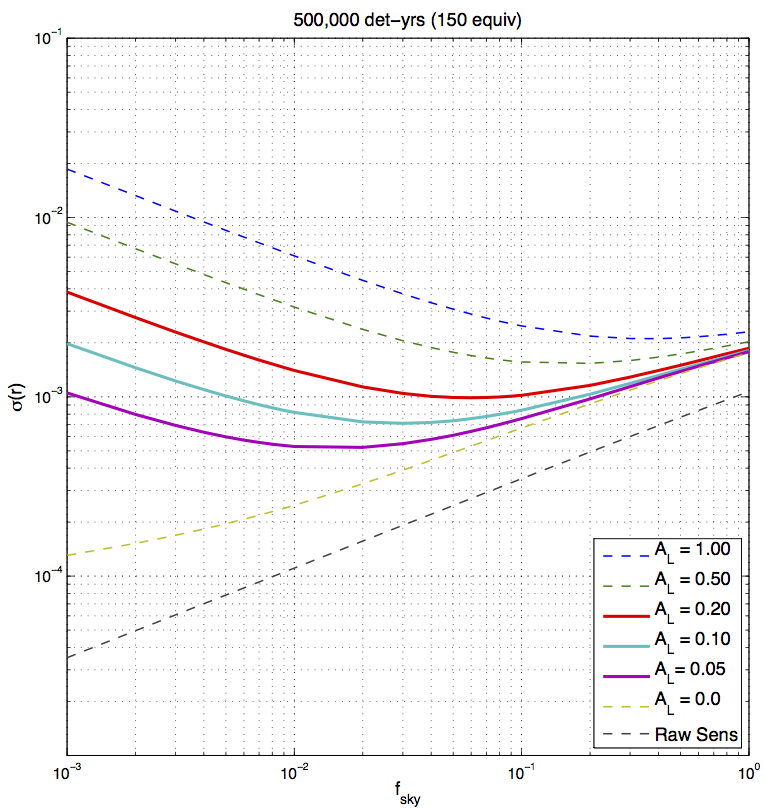
\includegraphics[width=0.49\textwidth]{Inflation/sigr2_fsky_rx1e3_r0.png}
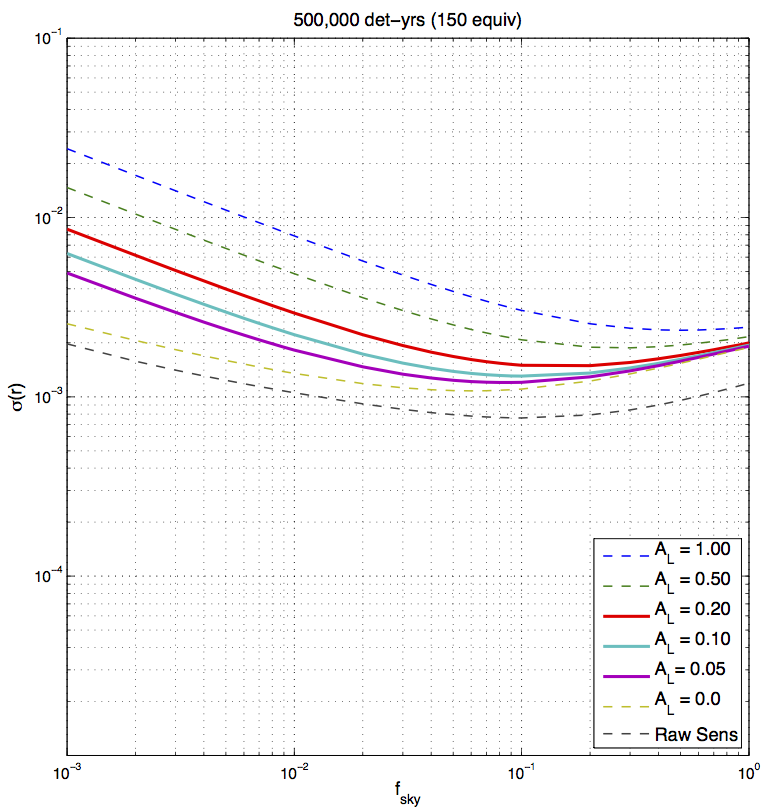
\includegraphics[width=0.49\textwidth]{Inflation/sigr2_fsky_rx1e3_r01.png}
\caption{Forecasted uncertainty on $r$, assuming $r=0$ (left panel) and $r=0.01$ (right panel). The forecasting procedure assumes
an amount of delensing achieved, so we show several cases from complete delensing ($A_{\rm L} = 0$) to no delensing ($A_{\rm L} = 1$). The cases $A_{\rm L} = 0.05$ to $0.2$ are highlighted as we expect what is achieved will be in this range.}
\label{fig_rforecast}
\end{figure}



\section{Improved constraints on primordial density perturbations}
\label{sec:scalar}
%CMB-S4 will either detect primordial gravitational waves or improve current constraints on the amplitude of their power spectrum by almost two orders of magnitude. In addition, CMB-S4 will significantly improve our knowledge of the statistical properties of primordial density perturbations. 
All current data are consistent with primordial density perturbations that are adiabatic, Gaussian, and nearly scale invariant. Because of its high angular resolution, CMB-S4 will significantly improve current constraints on the scale dependence of the primordial power spectrum of scalar perturbations, on departures from Gaussianity, and on departures from adiabatic perturbations. In fact, it will measure anisotropies in both the temperature and E-mode polarization of the CMB to cosmic variance over the entire range of multipoles that is not contaminated by unresolved foregrounds. As a consequence, it will place the strongest constraints achievable by any ground-based CMB experiment on all observables that benefit from the number of modes measured, such as the primordial power spectrum and higher order correlations.

\subsection{The power spectrum of primordial density perturbations}
%{\it The scalar spectral index}\\
The density perturbations are close to scale invariant but not exactly so. In the context of $\Lambda$CDM, {\it Planck} has measured the scalar spectral index to be $n_s=0.9677\pm0.0060$ and has established $n_s-1<0$ at more than $5\,\sigma$. CMB-S4 will improve current constraints on the spectral index by more than a factor two to $\sigma(n_s)=0.0028$, and will provide valuable constraints on the space of inflationary models. 

%{\it Running of the scalar spectral index}\\
As mentioned in section~\ref{sec:upperLimits}, a measurement of the running of the scalar spectral index with a precision of a few parts in ten thousand would allow a measurement of $p$ in equation~(\ref{eq:nsassump}), or equivalently $\mathcal{N}_\star$. This precision cannot be achieve with CMB-S4, but with a precision of one part in a thousand, it will test the idea that the lack of power on large angular scales might be explained by scale dependence of the spectral index~\cite{Meerburg:2014bpa}.  

%{\it Oscillations in the primordial power spectrum}\\
Models of inflation that achieve super-Planckian inflaton displacements from repeated circuits of a sub-Planckian fundamental period may give rise to oscillatory features in the spectrum or primordial perturbations. The features may arise either from instanton effects or from periodic bursts of particle or string production. A search for such features is well motivated even though the amplitude is model-dependent and may be undetectably small. A detection would provide clues about the microscopic origin of the inflaton, the absence of a detection can constrain the parameters space of these models in interesting ways. CMB-S4 would tighten the constraints on the amplitude of features in the primordial power spectrum by a factor three. 
 
\subsection{Higher order correlations}
Any detection of departures from Gaussianity would shed light on the interactions either of the inflaton with itself or between the inflaton and other degrees of freedom. The lowest order correlation function that encodes departures from Gaussianity is the $3pt$-function
\begin{equation}
\langle\zeta(\vec{k}_1)\zeta(\vec{k}_2)\zeta(\vec{k}_3)\rangle=(2\pi)^3\delta(\vec{k}_1+\vec{k}_2+\vec{k}_3)B(k_1,k_2,k_3)\,,
\end{equation}
where invariance under rotations and translations guarantee that the bispectrum $B(k_1,k_2,k_3)$ only depends on the magnitudes $k_1$, $k_2$, and $k_3$. A model independent search for the bispectrum, or equivalently the angular bispectrum $b_{\ell_1\ell_2\ell_3}$, is not computationally tractable, and in practice searches place constraints on the amplitudes $f_{\rm NL}$ of certain theoretically motivated functional forms, or shapes.

A detection of the most widely studied local shape would have far reaching theoretical implications. A detection of this shape would rule out all models of single clock inflation \cite{Creminelli:2004yq}. In addition, such a signal would open the door to significant cosmic variance on all scales from coupling of fluctuations within our observed volume to any super-Hubble modes \cite{Nelson:2012sb,LoVerde:2013xka,Nurmi:2013xv}. Indeed, there would be room for a significant shift between the observed amplitude of scalar fluctuations (and so the observed $r$) and the mean value of fluctuations on much larger scales. Any scenario that predicts local non-Gaussianity together with fluctuations on scales much larger than our observed volume predicts a probability distribution for our observed $f_{\rm NL}^{\rm local}$. Many well-motivated scenarios predict a small mean value. These include the simplest modulated reheating scenario \cite{Zaldarriaga:2003my} and ekpyrotic cosmology \cite{Lehners:2009ja}, both of which predict mean values of $f_{\rm NL}^{\rm local}\sim5$. 
Currently the strongest constraints on the local shape come from the {\it Planck} 2015 temperature and polarization analysis which give $f_{\rm NL}^{\rm local} = 0.8 \pm 5.0$~\cite{Ade:2015ava}. A noise-free cosmic variance limited CMB experiment is expected to produce constraints on $f_{\rm NL}^{\rm local}$ with 1$\sigma$ error bars of about 3 \cite{Komatsu:2001rj}. Therefore the improvement expected of CMB-S4 over current limits is slightly less than a factor of two. This is not sufficient to reach the interesting theoretical threshold around $|f_{\rm NL}^{\rm local}|\lesssim 1$~\cite{Alvarez:2014vva}, but will still reduce the space of viable models or hint at a detection. CMB-S4 could, for example, provide hints for the modulated reheating scenario or ekpyrotic cosmology at roughly $2\,\sigma$. The simplest curvaton scenario, which predicts $f_{\rm NL} = -5/4$ \cite{Lyth:2001nq}, will unfortunately be out of reach.

In models with a single clock, the symmetry breaking pattern underlying inflation guarantees that the fluctuations are governed by the action
\begin{equation}
S=\int\,d^4 x \sqrt{-g}\left[-\frac{M_p^2 \dot{H}}{c_s^2}\left(\dot{\pi}^2-c_s^2\frac{(\partial_i\pi)^2}{a^2}\right)+M_p^2 \dot{H}\left(1-\frac{1}{c_s^2}\right)\left(\dot\pi^3-\dot\pi\frac{(\partial_i\pi)^2}{a^2}\right)+M_3^4\dot\pi^3+\dots\right]\,,
\end{equation}
where at leading order $\zeta=H\pi$ and the omissions represent terms higher order in fields, derivatives, or both. In the presence of an approximate continuous shift symmetry, the coefficients in this action are approximately constant in time and there are only two linearly independent shapes. 
Current constraints on the equilateral and orthogonal shapes are $f_{\rm NL}^{\rm equil} = -4 \pm 43$ and $f_{\rm NL}^{\rm ortho} = -26 \pm 21$, both (68\% CL)~\cite{Ade:2015ava}. Because of its high angular resolution, CMB-S4 can improve these constraints by about a factor two which would further tighten existing constraints on the speed of sound during inflation and the strong coupling scale in single-clock models of inflation. In addition, the tighter constraints on the equilateral shape would constrain scenarios with secondary production of gravitational waves.

Especially in models in which the inflaton is an axion, there is only an approximate discrete shift symmetry. In these models instanton contributions to the potential and periodic bursts of particle or string production naturally lead to periodic features in the bispectrum. If moduli in the underlying string constructions do not evolve appreciably, instanton contributions lead to oscillations with a constant amplitude in the logarithm of $k$. In general, moduli evolve during inflation and cause a drift in the frequency and a scale-dependent amplitude~\cite{Flauger:2014ana}. At present, these shapes have not yet been constrained systematically. Often these contributions will lead to counter-parts in the power spectrum and are expected to be detected there first~\cite{Behbahani:2011it}, but this need not be the case~\cite{Behbahani:2012be}. So a search for these more general shapes is well motivated, and as for the scale invariant shapes CMB-S4 will improve constraints by about a factor two. 

{\bf (Beyond the bispectrum)}



%In the modulated reheating scenario, the field which drives inflation $\phi$ decays to the particles of the standard model with a rate $\gamma$ which is determined by the value of a second field $\sigma$ which remains light throughout inflation. The quantum fluctuations in $\sigma$ result in a spatially modulated reheating surface resulting in the curvature perturbations that we observe in the CMB and large scale structure. The process by which the fluctuations in the light field are converted into curvature fluctuations naturally results in local non-Gaussianity given by $f_{\rm NL} = 5(1-\Gamma \Gamma^{\prime\prime}/\Gamma^{\prime2})$, where this formula holds in the case that $\phi$ oscillates about a quadratic minimum after inflation and the fluctuations in $\phi$ make a negligible contribution to the observed power spectrum.

%This can be contrasted with the simplest curvaton scenario, where a scalar field $\sigma$ which remains light during inflation comes to dominate the energy density of the universe after the field which drives inflation $\phi$ decays. The fluctuations in the energy density of $\sigma$ then determine the curvature perturbations that are observed today. The local non-Gaussianity in this simple model is predicted to be $f_{\rm NL} = -5/4$ \cite{Lyth:2001nq}, which is unfortunately a few times smaller than the expected error bar from CMB Stage-IV.

%In the absence of a detection, however, it is important to ask what can be learned from improved constraints on $f_{\rm NL}$. Though not firm, nor entirely robustly defined, it can be argued that a natural theoretical threshold where qualitatively new general conclusions about the physics of the early universe can be drawn would come from constraints on $f_{\rm NL}<\mathcal{O}(1)$, see for example [1412.4671] for a detailed discussion. In order to achieve this level of constraint, it seems necessary to move beyond the cosmic microwave background to study other data sets, such as large scale structure. Despite the fact that CMB Stage-IV is not expected to reach this threshold, it is worth asking what can be gleaned from an improved constraint on $f_{\rm NL}$ from the CMB.


\subsection{Isocurvature}
{\bf To be added}




\section{Constraints on spatial curvature, birefringence, cosmic strings, axions\dots}
\label{sec:other_topics}

\subsection{Spatial Curvature}

Despite the fact that inflation drives the spatial curvature to zero at the level of the background evolution, it predicts small, but non-zero curvature for a typical observer. The curvature measured in a Hubble patch receives contributions from long wavelength perturbations and is expected to be $|\Omega_k|<10^{-4}$. A measurements of $\Omega_k$ exceeding this expectation would contain important information about the process responsible for inflation. In particular, if $|\Omega_k|$ is found to be considerably larger than this value, it would tell us that the inflaton was not slowly rolling when scales slightly larger than our observable horizon exited the horizon. Furthermore, observations of large negative $\Omega_k$ would falsify eternal inflation, while observation of positive and large $\Omega_k$ would be consistent with false vacuum eternal inflation~\cite{Guth:2012ww,Kleban:2012ph}.

Current constraints on this parameter from the CMB alone are $\Omega_k= 0.005^{+0.016}_{-0.017}$. Including baryon acoustic oscillation (BAO) data tightens the bound to $\Omega_k=0.000\pm0.005$. CMB-S4 is expected to constrain spatial curvature at a level of $\sigma(\Omega_k)\approx 10^{-3}$. A detection at this level would have profound implications for the inflationary paradigm. 



\subsection{Cosmic Birefringence}
The simplest dynamical way to model the accelerated expansion of the universe is to invoke a new slowly evolving scalar field that dominates its energy budget (the quintessence models for DE). Such a field generically couples to photons through the Chern-Simons term in the electromagnetic Lagrangian, causing linear polarization of photons propagating cosmological distances to rotate---the effect known as cosmic birefringence~\cite{1998PhRvL..81.3067C}. In the case of the CMB, such rotation converts the primordial E mode into B mode, producing characteristic TB and EB cross-correlations in the CMB maps \cite{2009PhRvL.102k1302K,2009PhRvD..80b3510G}. Even though there is no firm theoretical prediction for the size of this effect, if observed, it would be a clear “smoking-gun” evidence for physics beyond the standard model. Previous studies have used quadratic estimator formalism to constrain this effect \cite{2012PhRvD..86j3529G}, with the best current limit coming from sub-degree scale polarization measurements with POLARBEAR \cite{Ade:2015cao} ($<0.33$ deg$^2$ for the amplitude of a scale-invariant rotation-angle power spectrum). A promising way to pursue search for cosmic birefringence in the future is measurement of the off-diagonal EB cross correlations on small angular scales. {\bf Put in more specific predictions for S4?}

\subsection{Cosmic Strings}

Cosmic strings can at most contribute O(1\%) to the total CMB temperature anisotropy~\cite{Ade:2013xla,Lizarraga:2014xza,Lazanu:2014eya}, however, they can still generate observable B-modes. As shown in \cite{Moss:2014cra}, the bounds on cosmic strings obtained solely from the POLARBEAR \cite{Ade:2014afa} and BICEP2  \cite{Ade:2014xna} B-mode spectra are comparable to those from temperature spectra. CMB-S4 polawill be able to reveal the presence of cosmic strings through their B-mode signature even if strings contribute as little as 0.1\% to the CMB temperature anisotropy \cite{Avgoustidis:2011ax}. 

\subsection{Anomalies}

Several unexpected features have been observed in the temperature of the CMB sky at relatively low-l or large angular scales.  Some of these were first noticed in COBE data,  
and all have been seen in both WMAP and Planck maps.  These include: 
\begin{itemize}
  \item a lack of correlation on the largest angular scales;
  \item alignment of the lowest multipole moments with one another and with the geometry and motion of the Solar System;
  \item a hemispherical asymmetry or dipolar modulation of the power; 
  \item greater power in odd-parity modes than in even-parity ones.
\end{itemize}

Compared to the expectations of the best-fit inflationary $\Lambda$CDM model, the individual p-values of these features are in the per mille to per cent level, and therefore each anomaly has a frequentist probability at approximately the 3-sigma level or higher.  Since certain pairs of anomalies are uncorrelated in $\Lambda$CDM, in combination they nominally represents a very significant detection of anomalous behaviour. 

There are however two possible concerns before one can conclude that the CMB large-angle pattern is truly anomalous. First, these features were identified a posteriori and are characterized by statistics that were devised after the anomalies were first noted. Second, there is no physical understanding of how the collection of such features could arise. In order to help address or resolve these concerns, it is therefore crucial to obtain additional information about the large-scale primordial fluctuations, and to devise a successful model or other explanation.

The observed features can have two possible origins: either our cosmological model is incomplete and requires a modification (the “new physics hypothesis”), or we just happen to live in a realization of that model that is statistically unlikely (the “fluke hypothesis”).   Meanwhile, cosmologists have effectively exhausted their ability to obtain further independent CMB temperature data that can test these anomalies, as observations are already cosmic-variance limited at the relevant angular scales.

It has been suggested that one may nevertheless make observational progress, at least in the frequentist sense, even in the absence of an alternative model.  This can occur in two ways:
\begin{enumerate}
  \item In the fluke hypothesis the conditional probability distributions of $\Lambda$CDM for correlation functions of CMB polarization
  (and other observables) with CMB temperature and with one another are altered by the observed temperature anomalies  
  (Dvorkin et al 2008, Copi et al 2013, Yoho et al. 2013). 
  \item In the new physics hypothesis, a given phenomenological model that explains the anomalies will have observational consequences
  for other observable quantities [Yoho et al. 2015]. For example, the absence of large-angle correlations in T may reflect a lack of
  long-distance correlation in a fundamental physical quantity like the potential; similarly, 
  a hemispherical asymmetry in TT power could cause a similar asymmetry in EE.
\end{enumerate}

A variety of ideas have been proposed to explain the anomalies, ranging from Solar system dust artifacts to anisotropic models of inflation (for a summary, see Copi et al, 2016). Unfortunately, none of those ideas lead to a convincing explanation, as it is simply difficult to find models that explain the alignments of the largest primordial structures in the universe while at the same time lowering the amplitude of large-angle temperature correlations (e.g. Gordon et al, 2005). 

Additional information from polarization on the largest angular scales would be of great help. Polarization probes only those epochs where a large number of free electrons saw a temperature quadrupole, i.e. just at photon decoupling and later at reionization, whereas the intensity maps probe the complete line of sight to the last scattering surface.
 
To give two examples: If the lack of correlation is an intrinsic property of the inflationary power spectrum, then it should be reflected by a suppression of the reionization bump in the polarization. And if the observed alignments are due to some nearby superclusters and voids, then the supercluster plasma might also leave its imprint on the polarization. 

S4, alone or in combination with other data, can begin to explore both the cosmological and the fluke explanation for the origin of the observed anomalies.  For example, $\Lambda$CDM instructs us how to remove the part of the E-mode signal that is correlated to temperature; the remainder should be Gaussian random and statistically isotropic.  If it contains a hemispherical anomaly (especially one aligned with the temperature asymmetry), that would be evidence against the fluke hypothesis [Copi, Knox, O’Dwyer and Starkman, contribution to March 9/10 S4 meeting, in preparation]. 

{\bf Add connections to axion physics. eg 1601.03049}
%%
%% Populate the .bib file with entries from SPIRES Bibtex (preferred)
%% or ADS Bibtex (if no SPIRES entry).
%%  SPIRES will also supply the CITATION line information; please include it.
%%

\section{Summary}
CMB-S4 is an ideal tool to test the inflationary paradigm and competing theories of the early universe. On the one hand, its exquisite sensitivity will allow a detection of degree scale B-modes in the CMB or achieve upper limits on the amount of B-mode polarization that improve current constraints on the tensor-to-scalar ratio by almost two orders of magnitude. In particular, it is sensitive enough to detect the level of B-mode polarization predicted in a wide range of well-motivated inflationary models. In doing so, it would provide invaluable information about physics at energy scales far outside the reach of any terrestrial particle physics experiment. In the absence of a detection it would exclude large classes of inflationary models. On the other hand, with its high angular resolution, it will measure anisotropies in both the temperature and E-mode polarization of the CMB to cosmic variance over the entire range of multipoles that is not contaminated by unresolved foregrounds, and it will extend our window to the early universe by almost one $e$-fold beyond the reach of current experiments. As a consequence, it will provide the best constraints achievable by any ground-based CMB experiment on any observable that benefits from the number of modes measured, such as the primordial power spectrum, and hence the spectral index, its running, features in the power spectrum, as well as higher order correlations.


 
